\section{ Bin averaging correction}
When calculating the cross section, an average
in each bin occurs (see \F{fig:bin}. If the cross section distribution
is linear in all variables inside the bins then the value
at center corresponds to the value obtained. This is not the case 
in the more realistic situation when the data distribution
has some structure inside the bin. 

\begin{figure}[h]
\begin{center}
 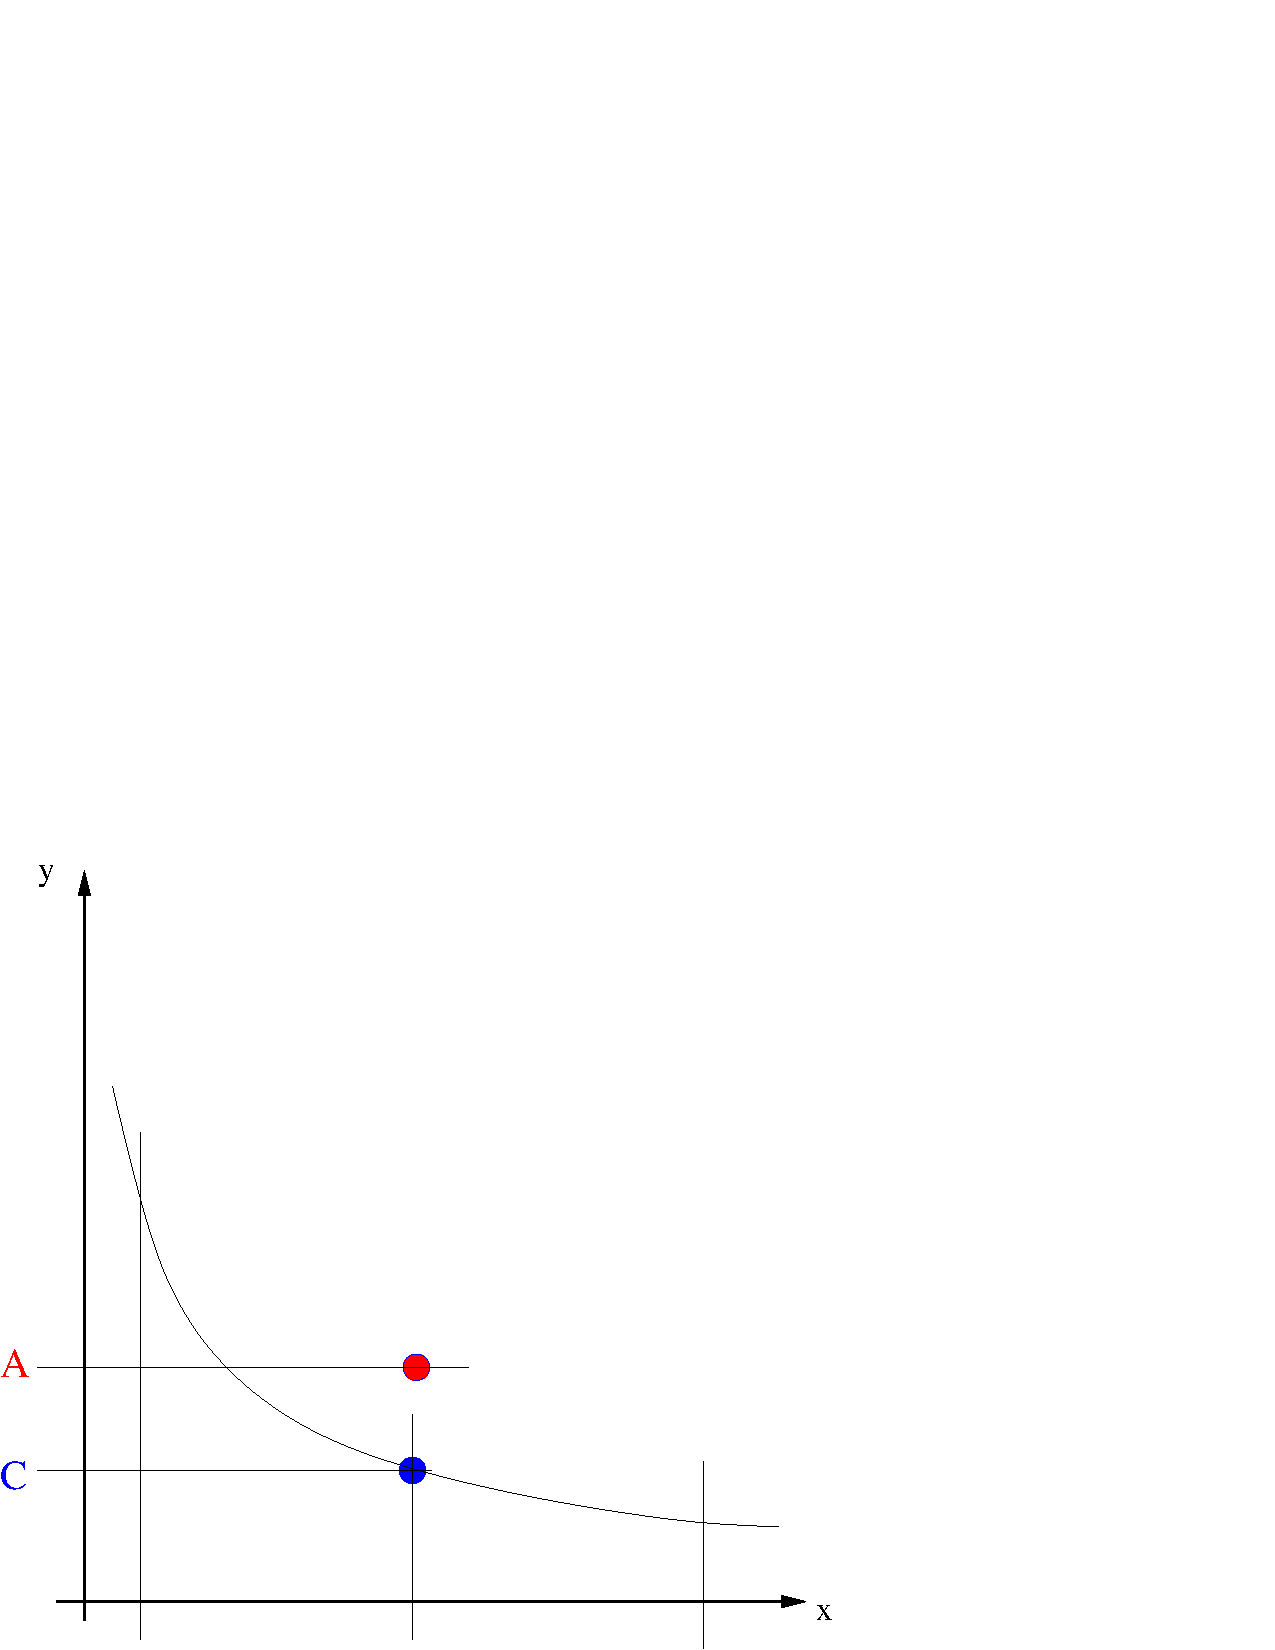
\includegraphics[width = 9cm, bb=-20 0 440 420]{analysis/img/bin}
  \caption[The bin correction]
          { The bin correction. $C$ is the value of the cross section at the center
	             of the bin, while $A$ is its average in that bin. The correction is $R=A/C$.}
 \label{fig:bin}
\end{center}
\end{figure}



To take in account this effect 
each bin was divided into subdivisions. The cross section
in each subdivision (using a model) was calculated to obtain the average $A$ in that 
whole bin. 
The value at the center of the bin $C$ was calculated as well. The resulting correction is
$$
 R = \Dfrac{C}{A}
$$





The model {\bf maid 2000 extended} \cite{bib:maid2000} is used to calculate the correction.
Each of the $15\times7\times12\times10 = 12600$ bins is divided into $15^4 = 50625$ subdivisions
($15$ for each of the variables $W$, $Q^2$, $\cos\theta$, $\phi$).
This gives a total of $\sim 600$ million calculated cross section points.
The correction in each bin is
$$
 R_{w,\, q^2,\, \cos\theta,\, \phi} = \Dfrac{C_{w,\, q^2,\, \cos\theta,\, \phi}}{A_{w,\, q^2,\, \cos\theta,\, \phi}}
$$
\F{fig:bin_averaging} illustrates the correction as a function of $\cos\theta$, $\phi$ for 
different $Q^2$ bins at the peak of the $\Delta(1232)$ resonance.
\vspace{1cm}
\begin{figure}[h]
 \begin{minipage}{7cm} 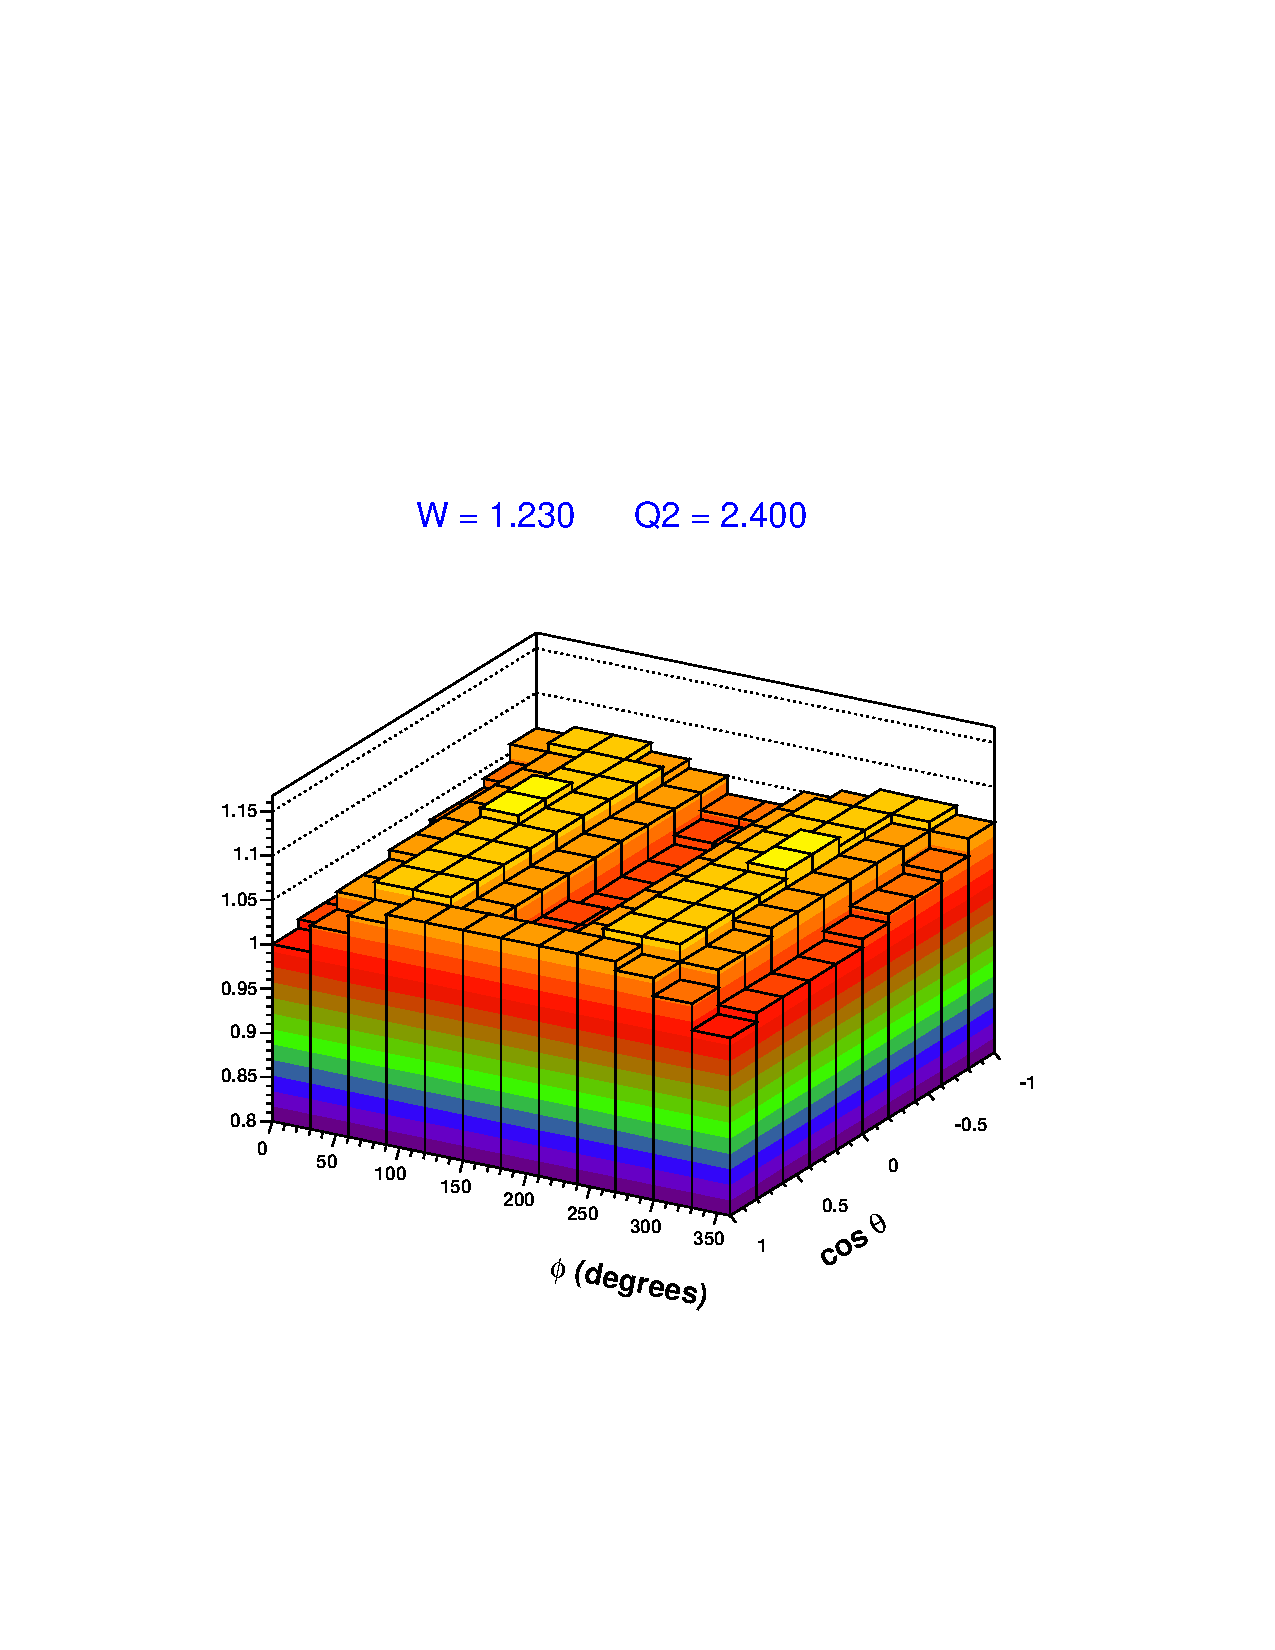
\includegraphics[width = 6.6cm, bb=60 130 520 570]{analysis/img/binave1} \end{minipage}
 \hspace{1cm}
 \begin{minipage}{7cm} 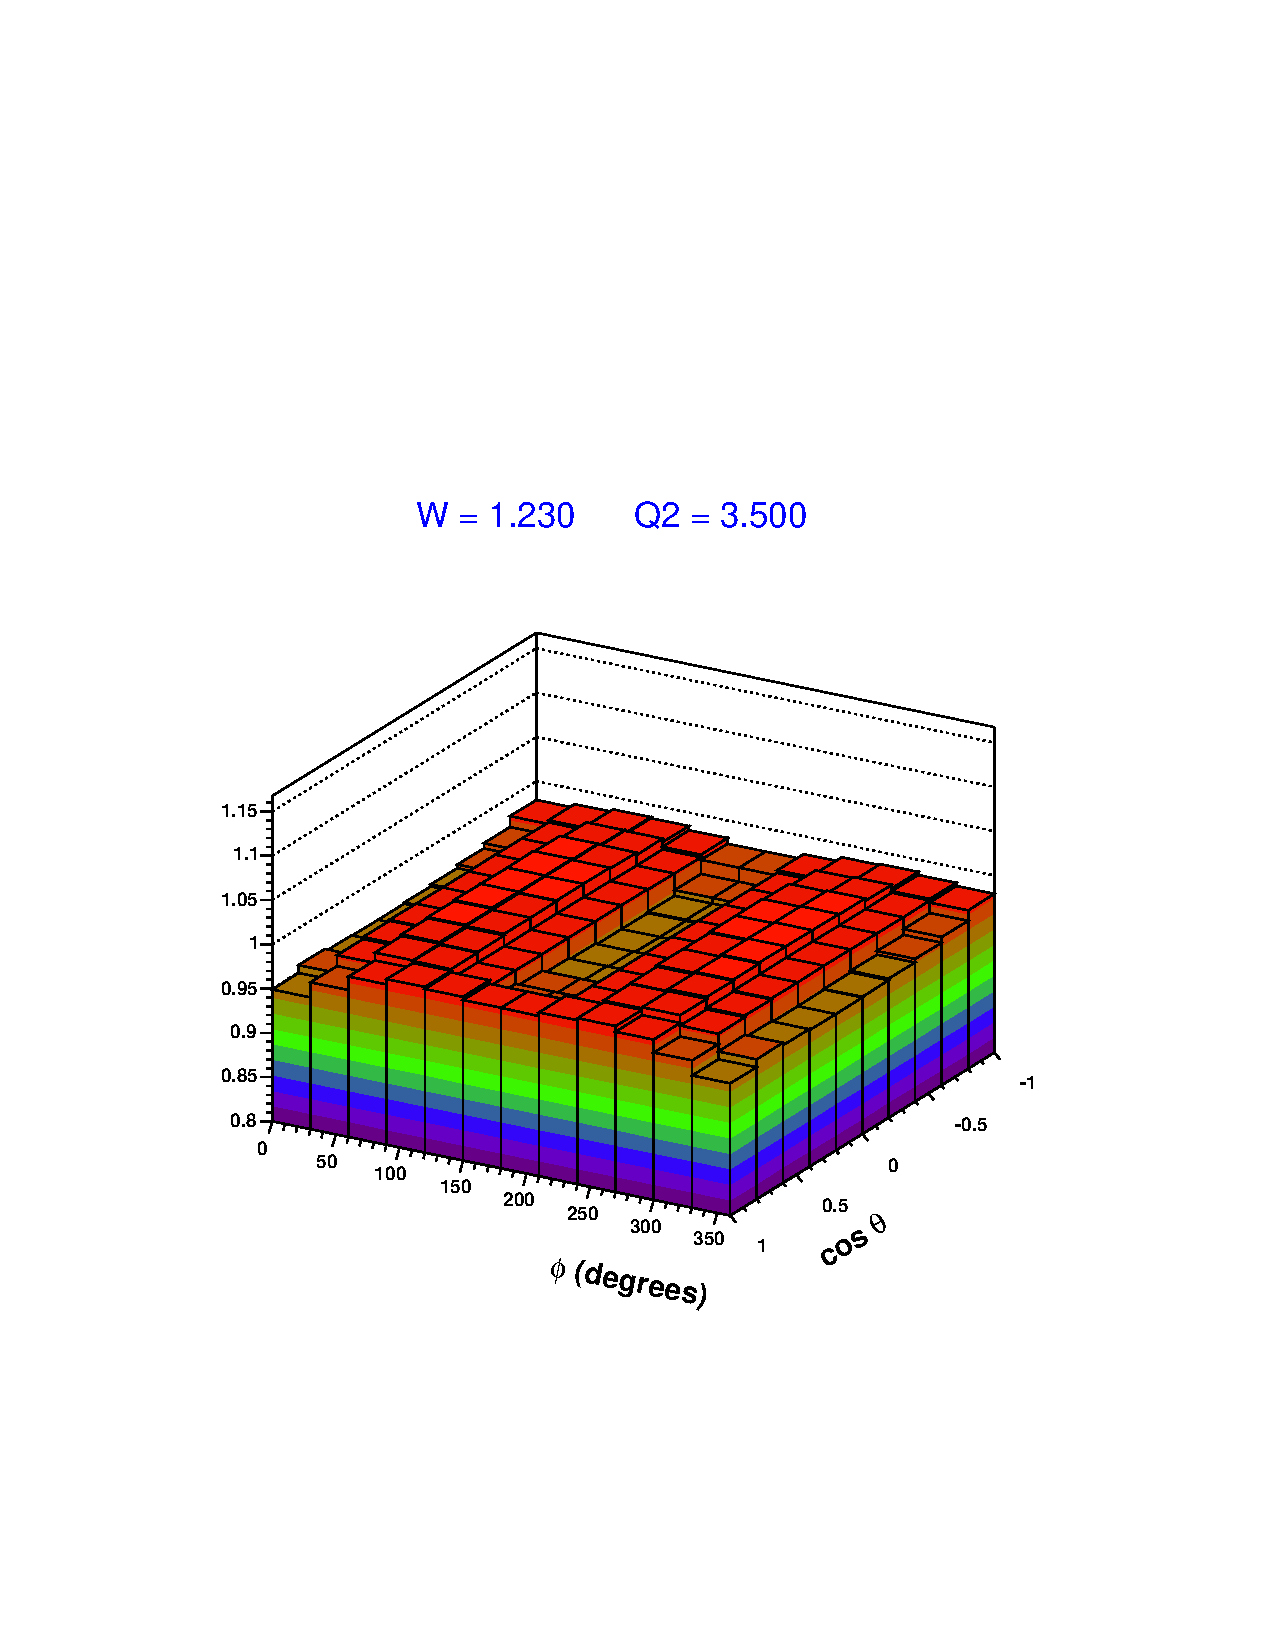
\includegraphics[width = 6.6cm, bb=60 130 520 570]{analysis/img/binave2} \end{minipage}  
 \\
 \vspace{0.1cm}
 \begin{minipage}{7cm} 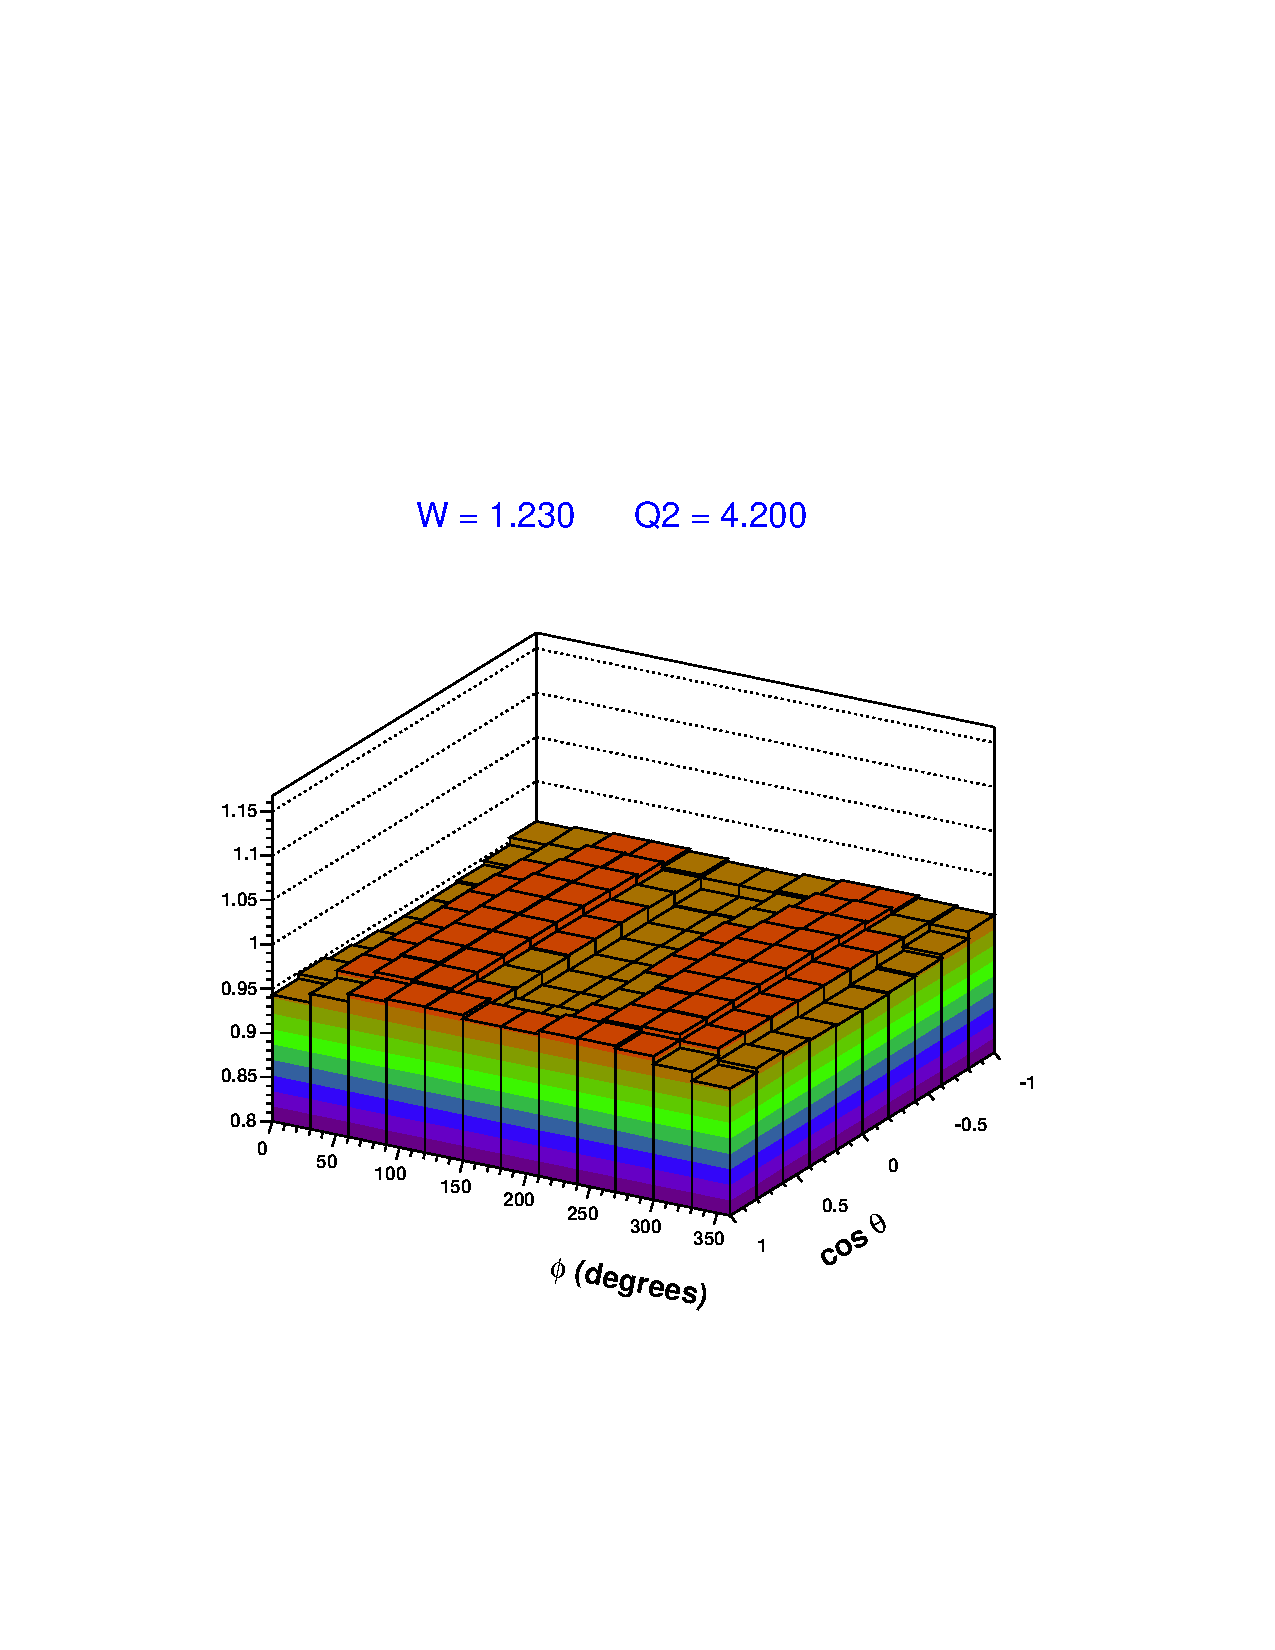
\includegraphics[width = 6.6cm, bb=60 130 520 570]{analysis/img/binave3} \end{minipage}
 \hspace{1cm}
 \begin{minipage}{7cm} 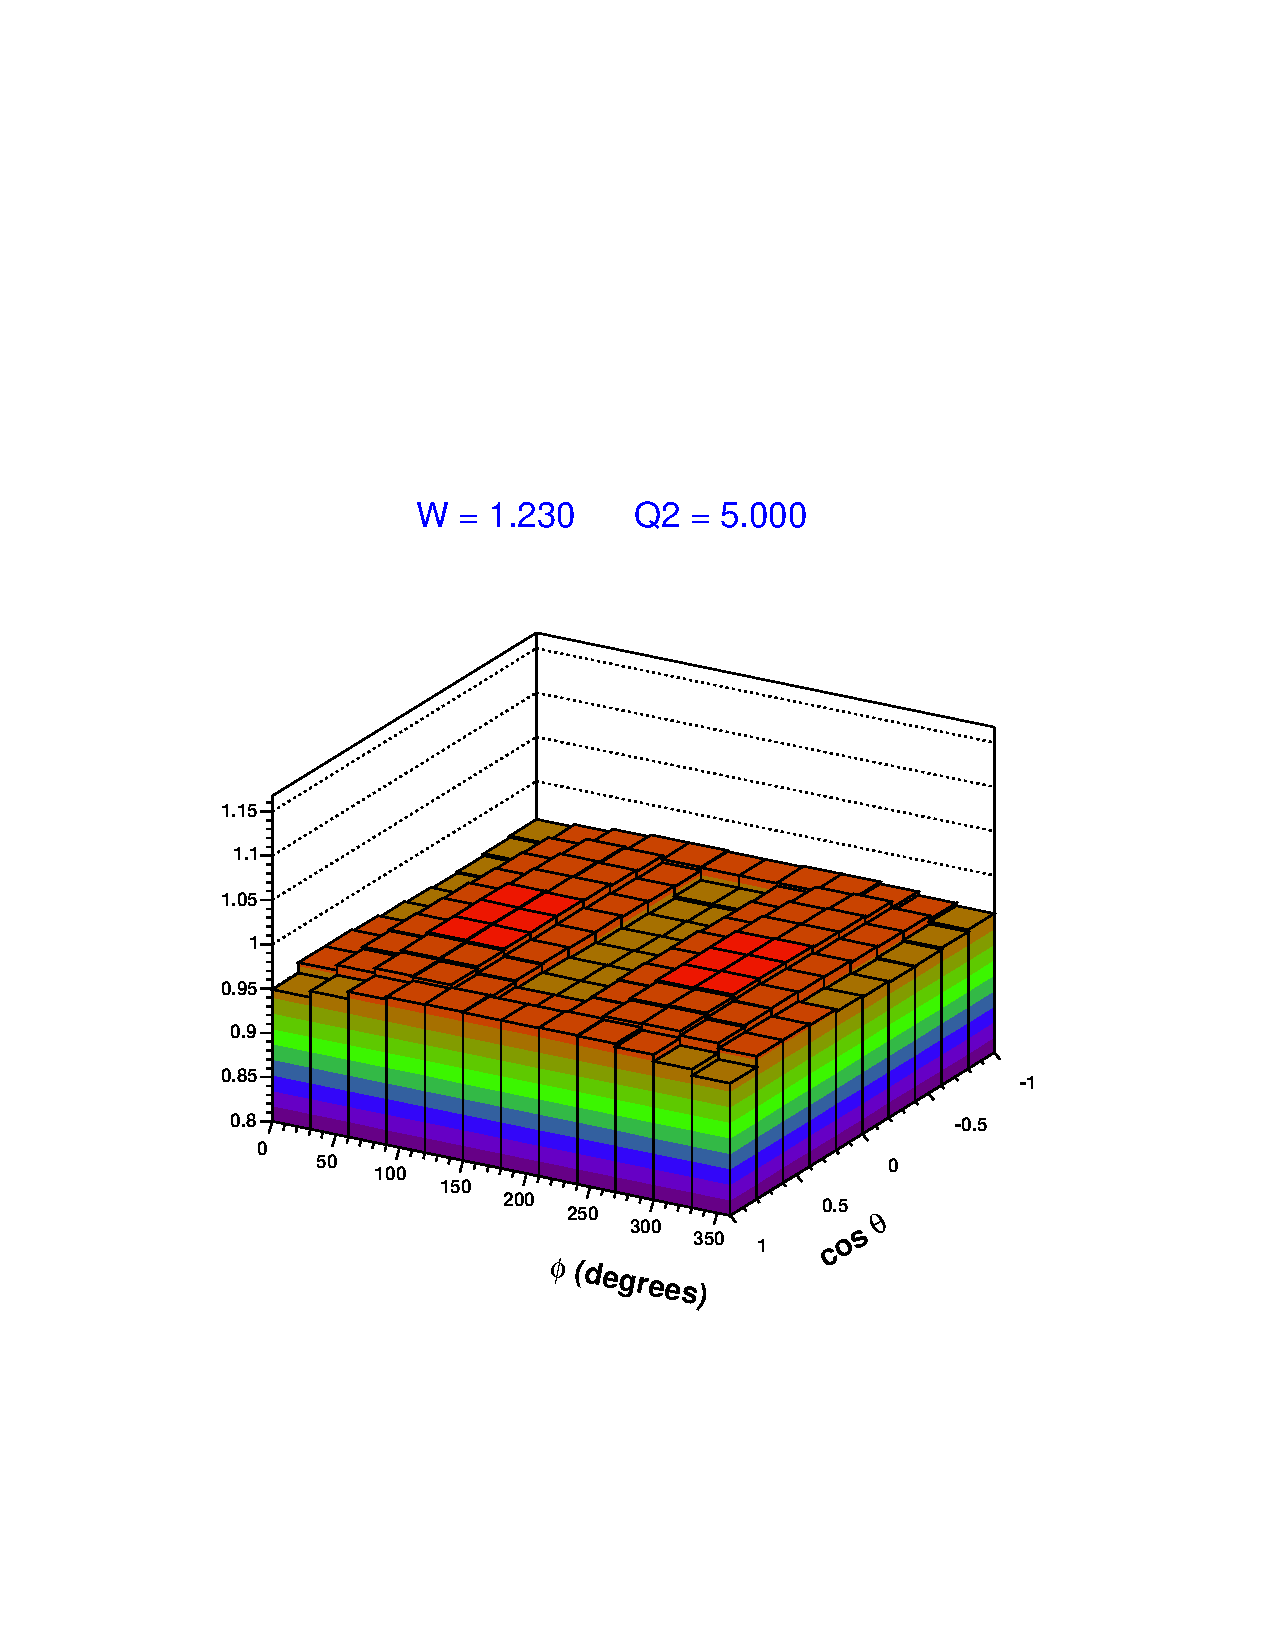
\includegraphics[width = 6.6cm, bb=60 130 520 570]{analysis/img/binave4} \end{minipage}    
  \caption
          { Bin averaging correction.}  
 \label{fig:bin_averaging}
\end{figure}  \\
See    \begin{verbatim} 
http://www.jlab.org/~ungaro/pi0eprod/bin_ave
\end{verbatim}
for the correction in each bin considered as a function of $\phi^*$ or $\cos\theta^*$.







